\documentclass[11pt]{article}
\usepackage{graphicx} 
\usepackage[margin=0.5in]{geometry}
\usepackage{helvet}
\renewcommand{\familydefault}{\sfdefault}
\linespread{1.3} 
\title{Dissertation Proposal : Quantifying the contributions of dispersal and niches to diversity maintenance in a microbial system}
\author{Amy Solman}
\date{27/11/2019}
\begin{document}
  \begin{titlepage}
   \begin{center}
       \vspace*{1cm}
 	\Huge
       \textbf{Dissertation Proposal}
 
       \vspace{0.5cm}
       \Huge
        Quantifying the contributions of dispersal and niches to diversity maintenance in a microbial system
 
       \vspace{1.5cm}
 	\huge
       \textbf{Amy Solman} \\
       amy.solman19@imperial.ac.uk
 
       \vfill
       \Large
 	Supervisors\\
         Tom Bell, Imperial College London, thomas.bell@imperial.ac.uk \\
        Ryan Chisholm, National University of Singapore, ryan.chis@gmail.com 
 
       \vspace{0.8cm}
 

 	\Large
       Department of Life Sciences\\
       Imperial College London\\
       27th November 2019
 
   \end{center}
\end{titlepage}
  
  \section{Keywords}
  Dispersal, niches, microorganisms, biodiversity, islands, biogeography

  \section{Introduction to the project idea and proposed questions}
  In 2016 Chisholm \textit{et al.}, published \textit{Maintenance of Biodiversity on Islands}\cite{chisholm2016maintenance}. The paper suggests that while the theory of Island Biogeography, proposed by MacArthur and Wilson \cite{wilson1967theory}, explains species-area relationships (SAR) for large islands, it fails to explain small islands for which SAR appears to be area independent. Chisholm \textit{et al.,} postulates that for small islands, ‘as island area increases, the total number of immigrants increases faster than niche diversity’. The theory explains that species richness on small islands follows a niche-structured regime, while large island biodiversity is dictated by colonization-extinction balance. This project will seek to experimentally test this hypothesis using microbial communities manipulated in the lab. 
  
  \section{Proposed methods}
  I propose to use several experimental treatments to mimic island conditions as described by Chisholm \textit{et al.,} including: varying ‘island’ areas, immigration rates and niche availability. Samples from a pre-populated 'mainland' microbial community will be applied to these sterile ‘island’ experimental treatments. After repeated population events the new 'island' microbial communities will be quantified using 16S rDNA sequencing. Species richness will be analysed to determine if there is a significant difference in community composition between experimental conditions. I will then attempt to fit the parsimonious mechanistic model used by Chisholm \textit{et al.,} to see if it significant explains any patterns of fluctuating diversity. If appropriate a range of models may be fit to the data.
  
  \section{Anticipated outputs and outcomes}
  Outputs: Dataset of microbial DNA sequences, used to identify community diversity; statistical analysis script (using Python/R) to assess any significant variation between the test communities; script to fit model(s) (possibly using High Performance Computing); final report. \\
Outcomes: We will have identified if the theories of Chisholm \textit{et al.,} were supported by our experimental data.

\section{Project feasibility supported by timeline of tasks}
All experimental work will be undertaken on-site at Silwood Park Campus under the supervision of Tom Bell. Theoretical support will also be provided by Ryan Chisholm. The proposed methods of this project, experimentally, analytically and computationally, are within the bounds of previous dissertations for this course. 
\begin{figure}[h!] 
	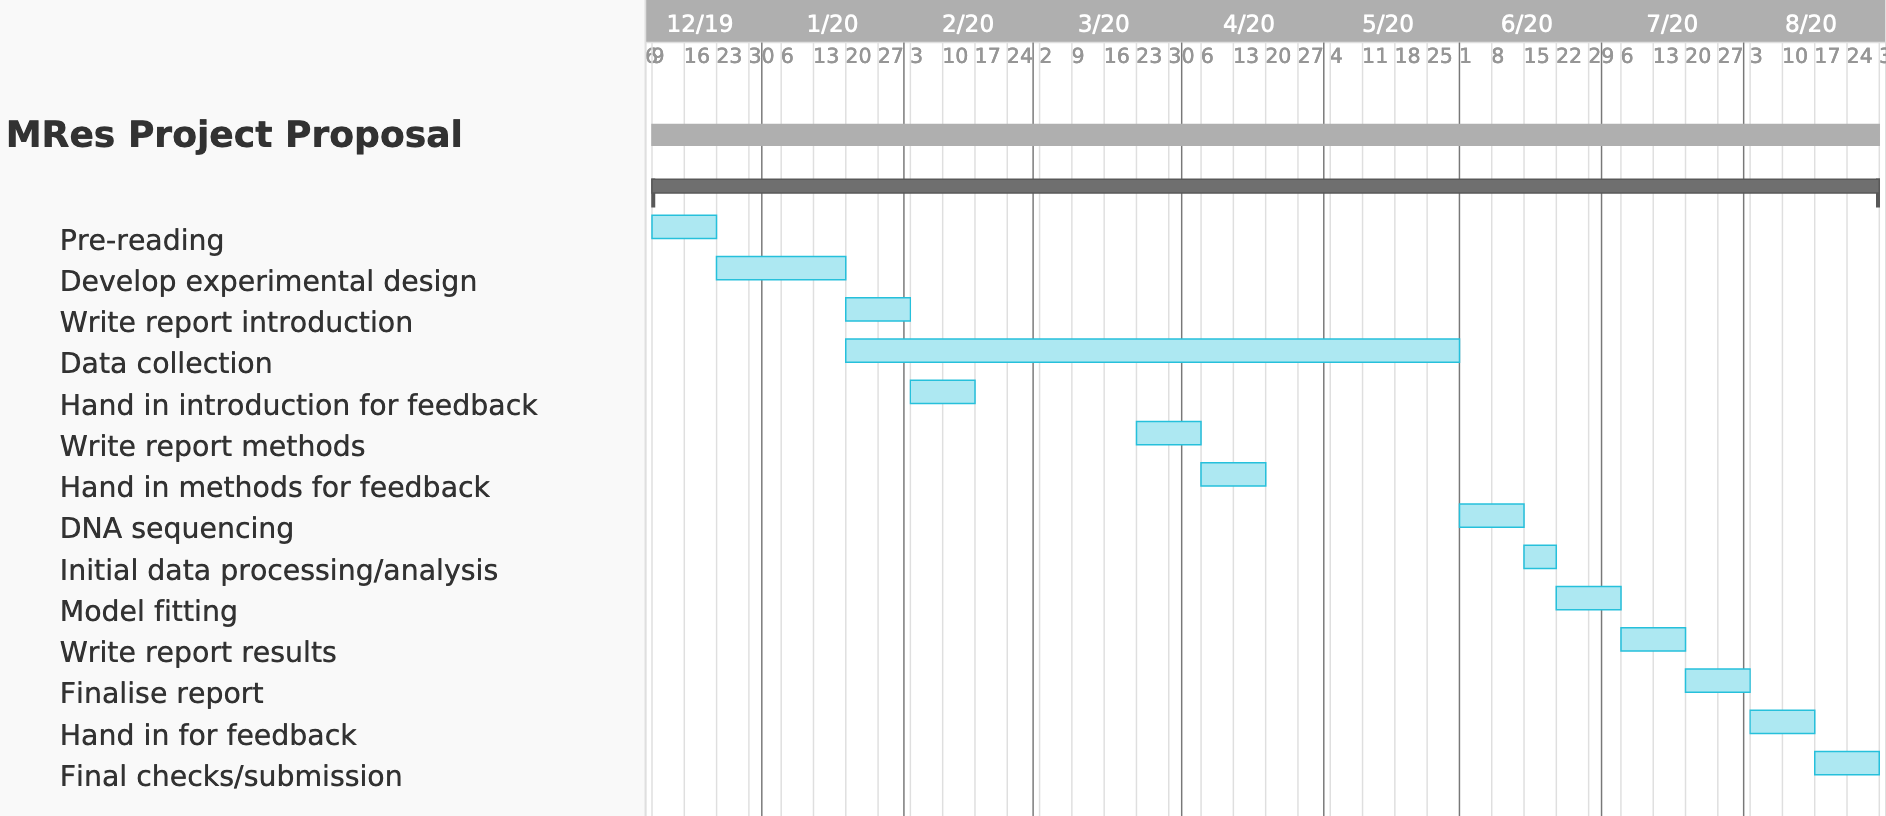
\includegraphics[width=\linewidth]{gantt_chart.png}
	\caption{Gantt chart of proposed project timeline Dec 2019 - August 2020} 
\end{figure}

\section{An itemized budget}
16S rDNA sequencing \\
Materials: Containers/substrate for experimental treatments \\
Access to High Performance Computing service 

  \bibliographystyle{plain}
  \bibliography{DissProp}
  
\end{document}